\documentclass{beamer}
\usepackage[utf8]{inputenc}
\usepackage[T1]{fontenc}
\usepackage[english]{babel}
\usepackage{graphicx}
\usepackage{times}

\usetheme{AGH}

\title[Praca inżynierska]{Aplikacja internetowa umożliwiająca wynajmowanie mieszkań oraz pokojów na rynku pierwotnym oraz wtórnym}

\author[P. Konsek]{Piotr Konsek}

\date[2015]{14.11.2015}

\institute[AGH]
{Informatyka\\ 
Wydział Elektrotechniki Automatyki Informatyki i Inżynierii\\
Biomedycznej
}

\setbeamertemplate{itemize item}{$\maltese$}

\begin{document}

{
%\usebackgroundtemplate{
\includegraphics[width=\paperwidth]{titlepage}} % wersja angielska
\usebackgroundtemplate{
\includegraphics[width=\paperwidth]{titlepagepl}} % wersja polska
 \begin{frame}
   \titlepage
 \end{frame}
}

%---------------------------------------------------------------------------


\begin{frame}
\frametitle{Agenda}
\begin{itemize}
\item Wstęp
\item Cel pracy
\item Użyte technologie
\item Implementacja
\item Wnioski
\item Zakończenie
\end{itemize}

\end{frame}

%---------------------------------------------------------------------------

\begin{frame}
\frametitle{Wstęp}
\begin{itemize}
\item Duże zainteresowanie społeczne zmianą miejsca zamieszkania zwłaszcza wśród osób młodych.
\item Brak wyspecjalizowanych darmowych serwisów w dziedzinie handlu nieruchomościami.
\item Nacisk ze strony użytkownika na szybkość i wygodę.
\end{itemize}

\end{frame}

%---------------------------------------------------------------------------


\begin{frame}
\frametitle{Cel pracy}
\begin{itemize}
\item Intuicyjny interfejs użytkownika
\item Bezpieczeństwo użytkownika
\item Personalizowanie ofert dla użytkowników
\item Stworzenie przyjaznego portalu dla użytkowników
\end{itemize}

\end{frame}

%---------------------------------------------------------------------------

\begin{frame}
\frametitle{Ruby on Rails}
\begin{itemize}
\item Framework powstał w 2005 roku
\item Szybkość pisania kodu oraz instalowania dodatkowych bibliotek
\item Elegancka składnia
\item Konwencja nazw ważniejsza niż konfiguracja
\item Wbudowany mechanizm ORM
\end{itemize}

\end{frame}

%---------------------------------------------------------------------------

\begin{frame}
\frametitle{Google Maps API}
\begin{itemize}
\item Bezpłatna usługa jeżeli serwis z niego korzystający jest darmowy.
\item Łatwa integracja z istniejącą aplikacją
\item Możliwość dodawania znaczników, zaznaczania obszaru
\item Najpopularniejszy serwis z mapami w sieci
\end{itemize}

\end{frame}

%---------------------------------------------------------------------------

\begin{frame}
\frametitle{Implementacja - architektura}
\centerline{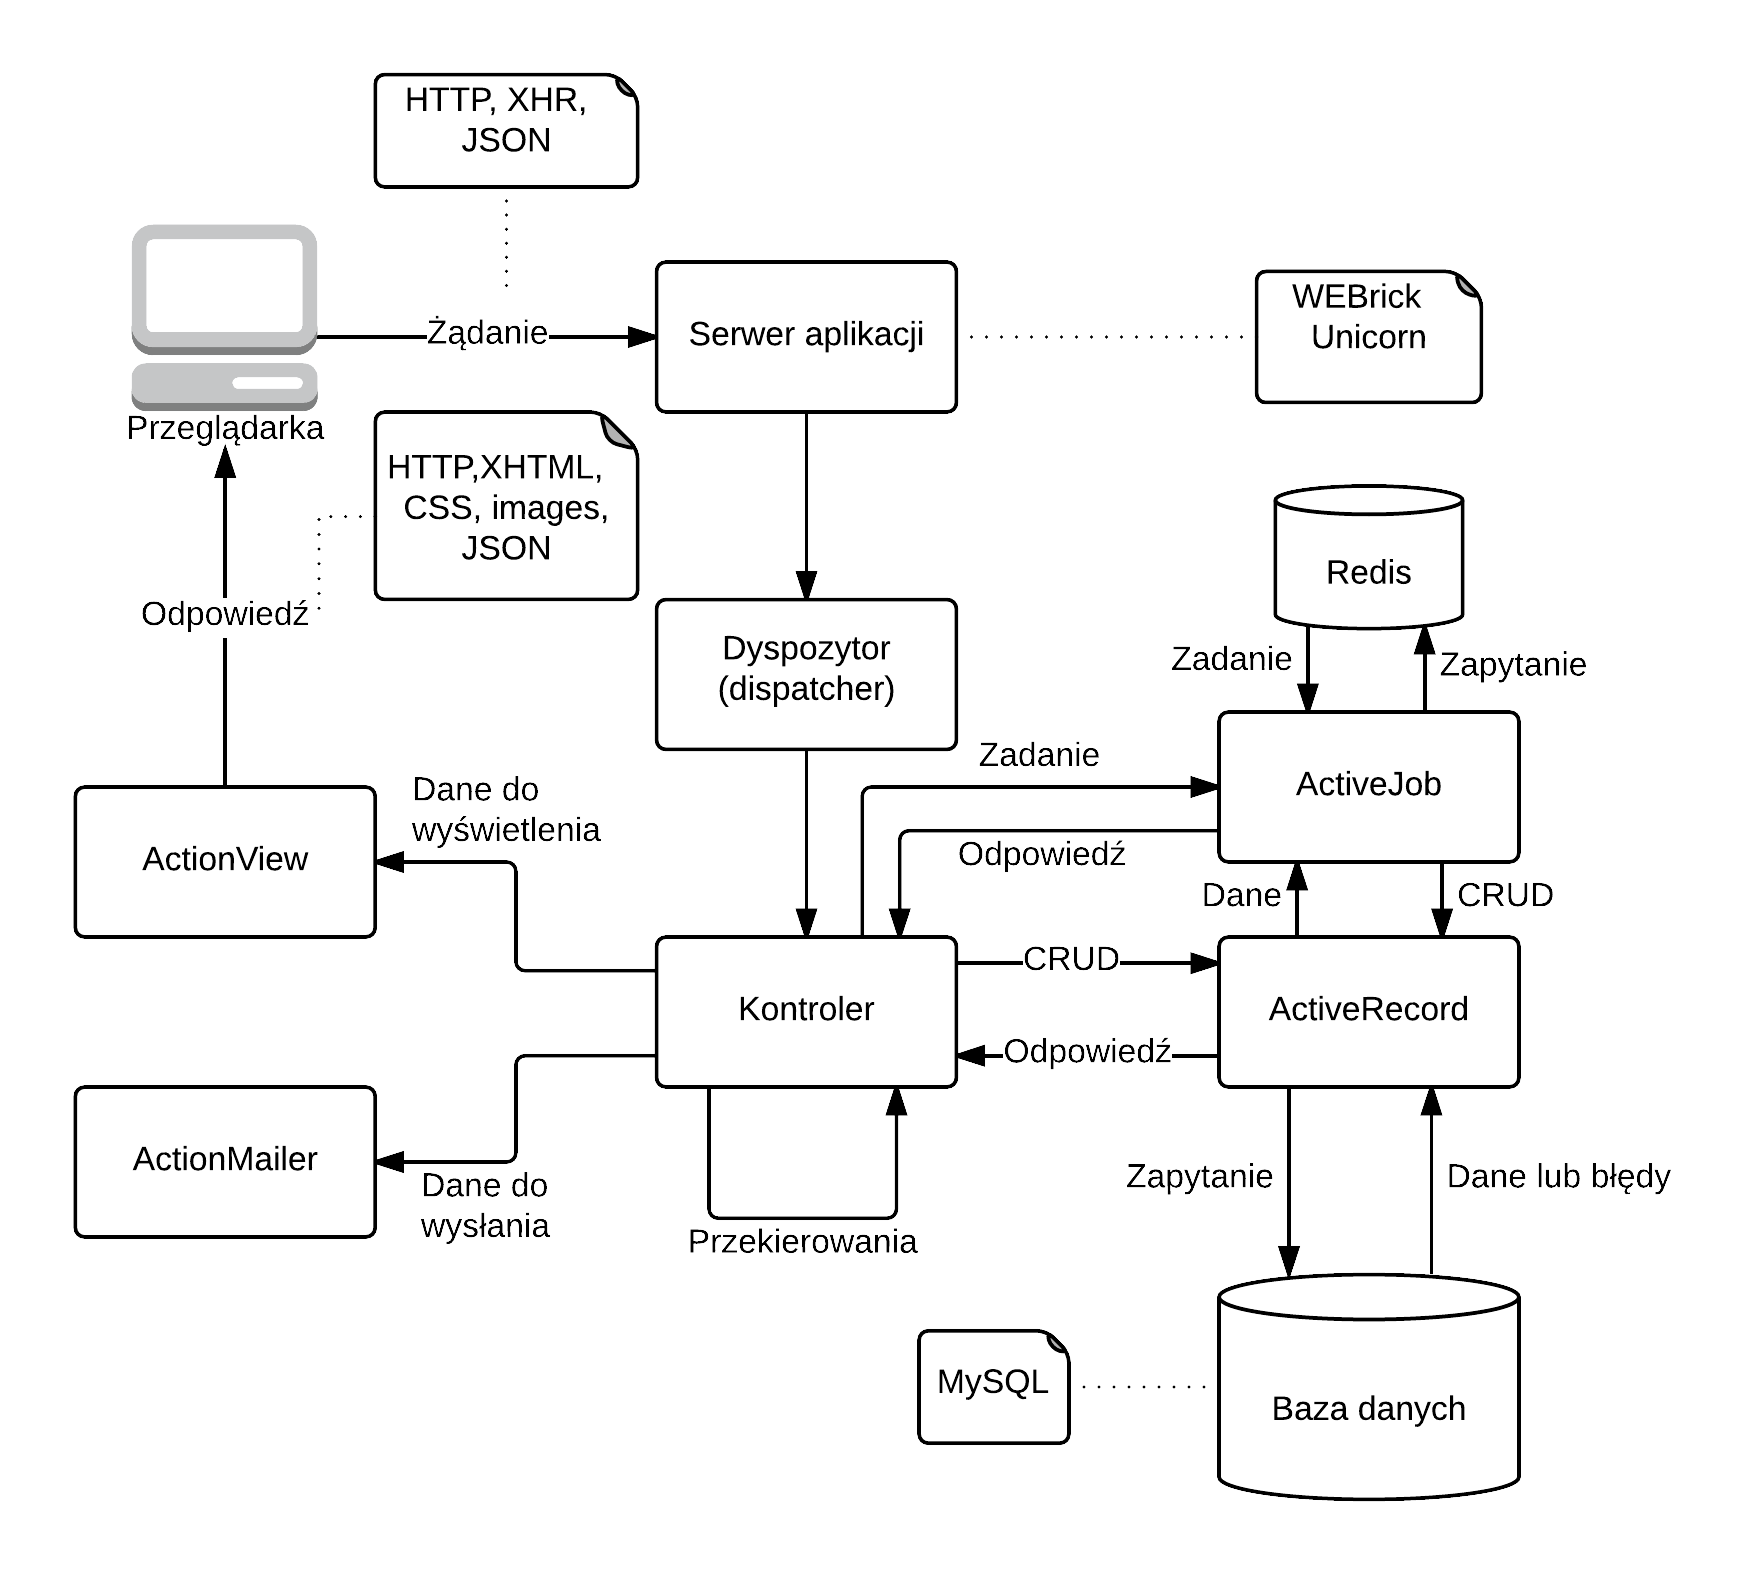
\includegraphics[scale=0.5]{pictures/architecture.png}}
\end{frame}

%---------------------------------------------------------------------------

\begin{frame}
\frametitle{Implementacja - główna strona}
\centerline{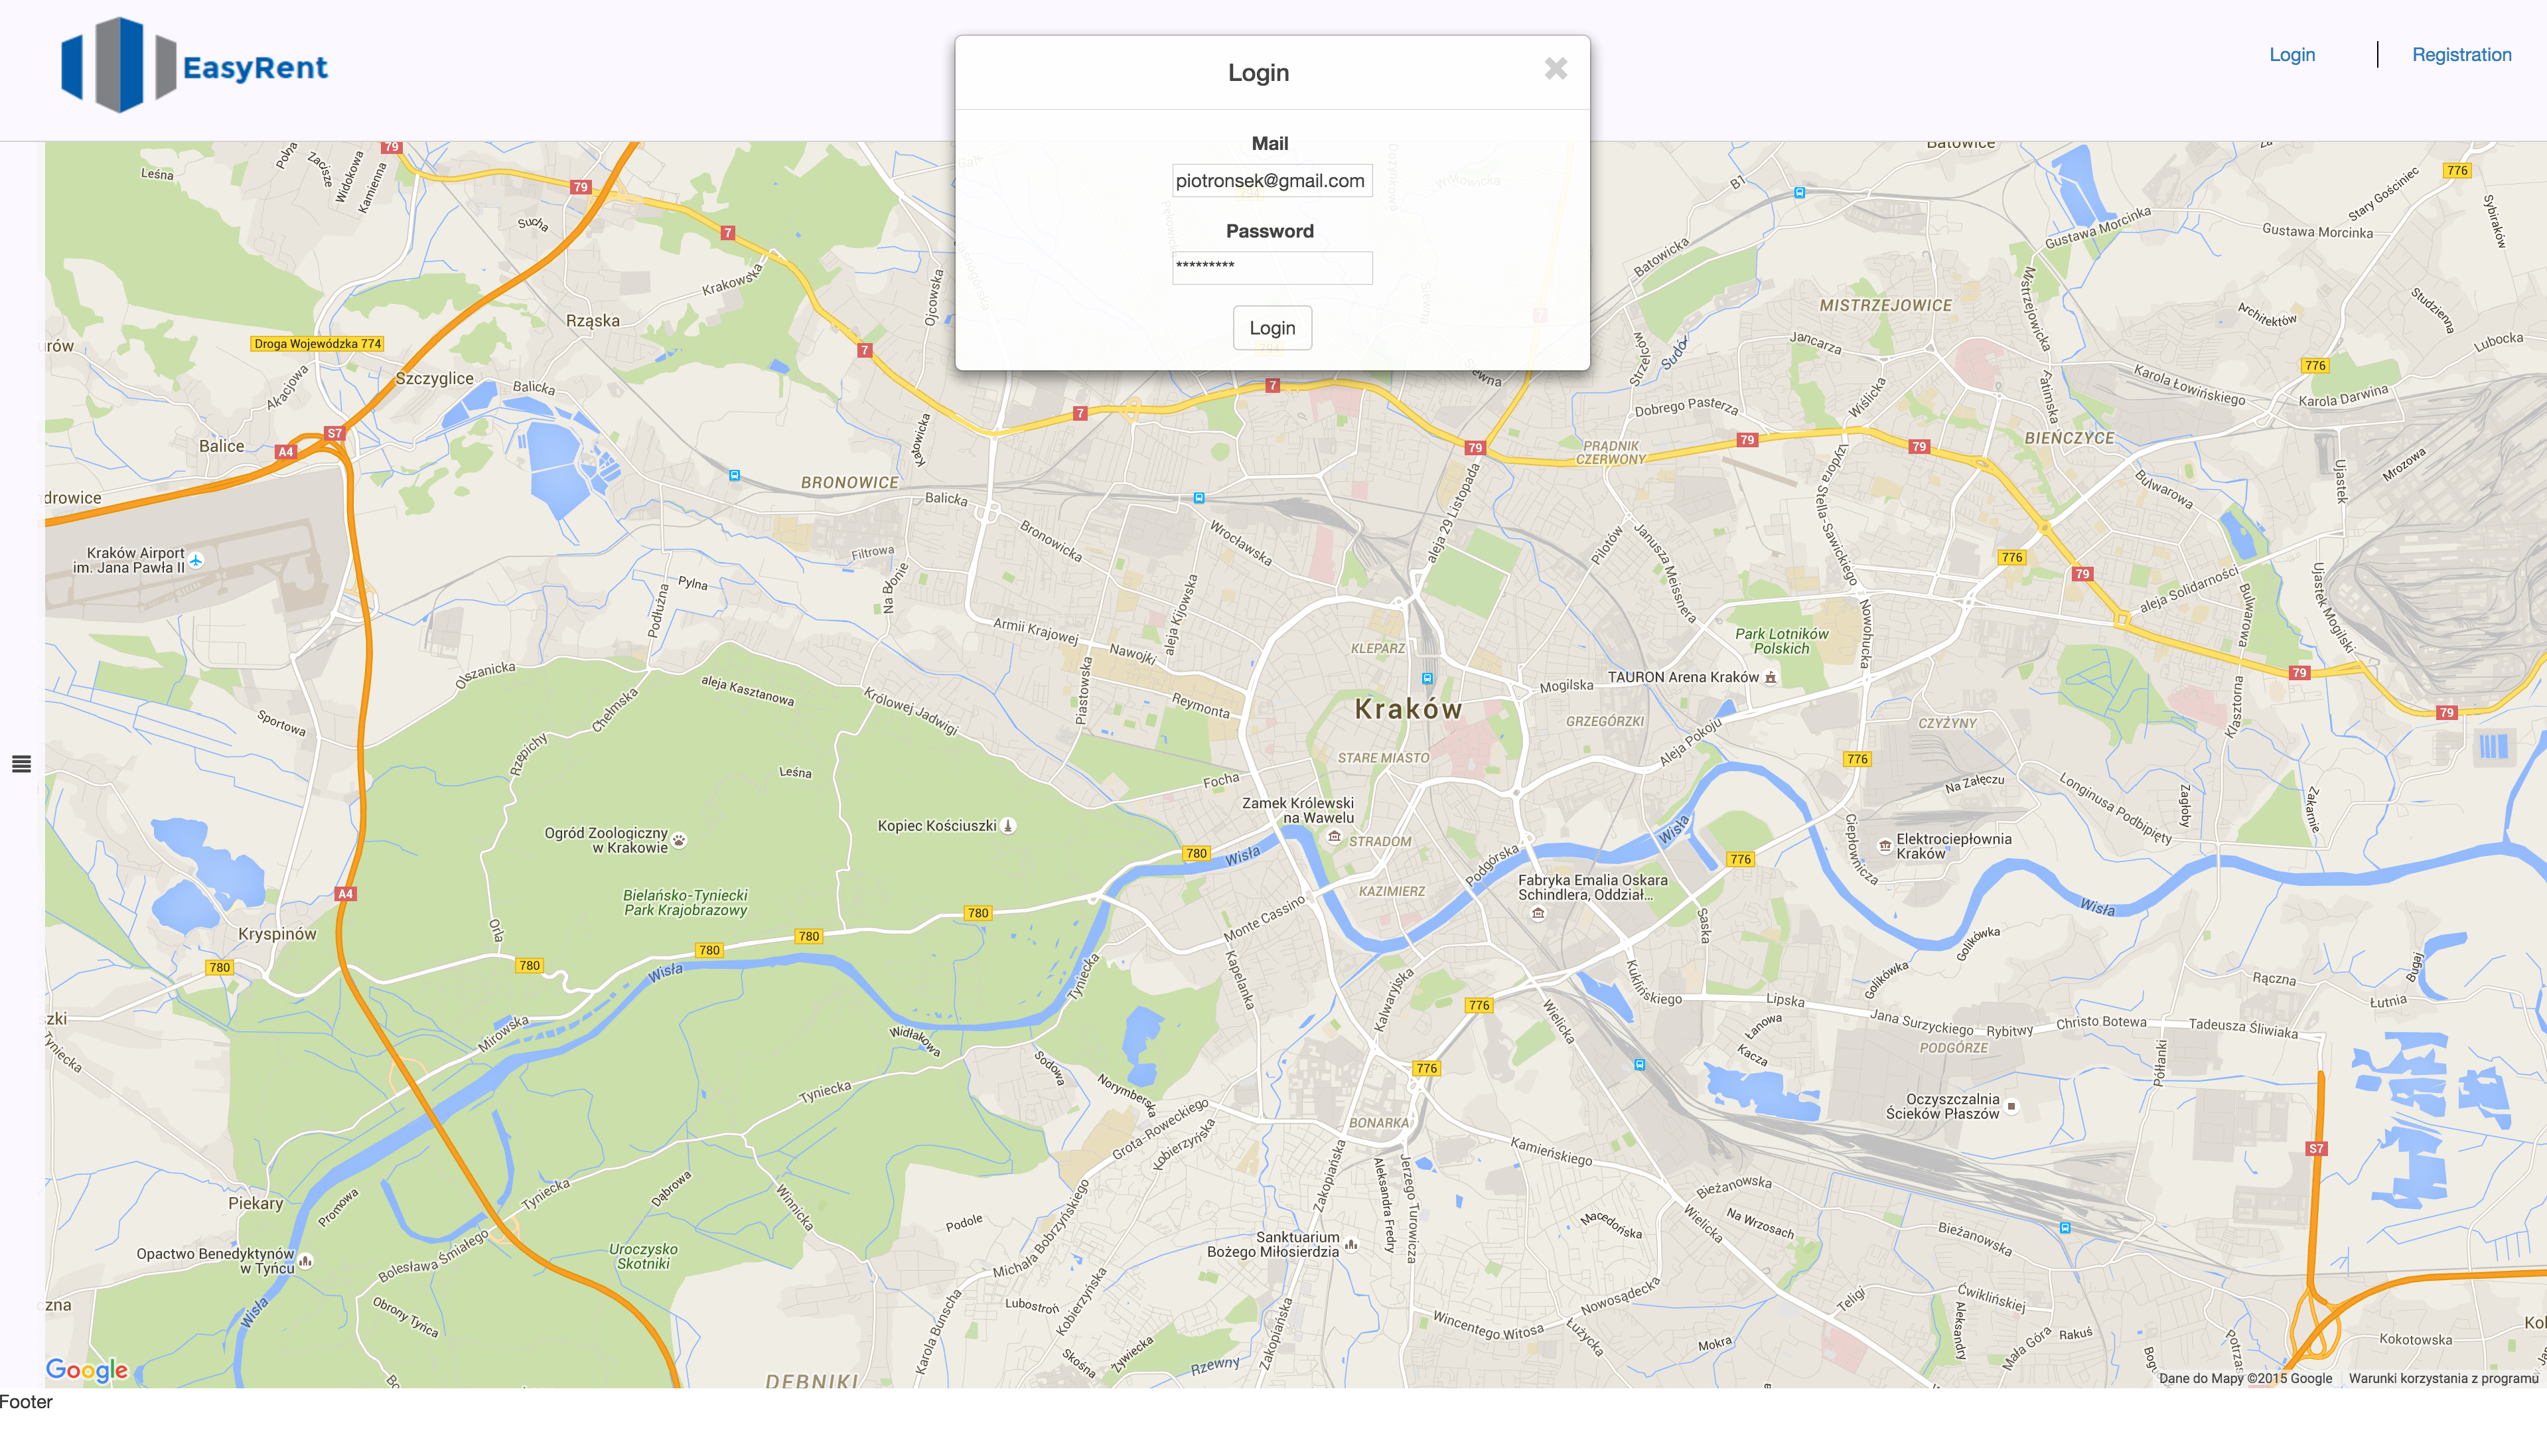
\includegraphics[scale=0.15]{pictures/before_login.png}}
\end{frame}

%---------------------------------------------------------------------------

\begin{frame}
\frametitle{Implementacja - filtry}
\centerline{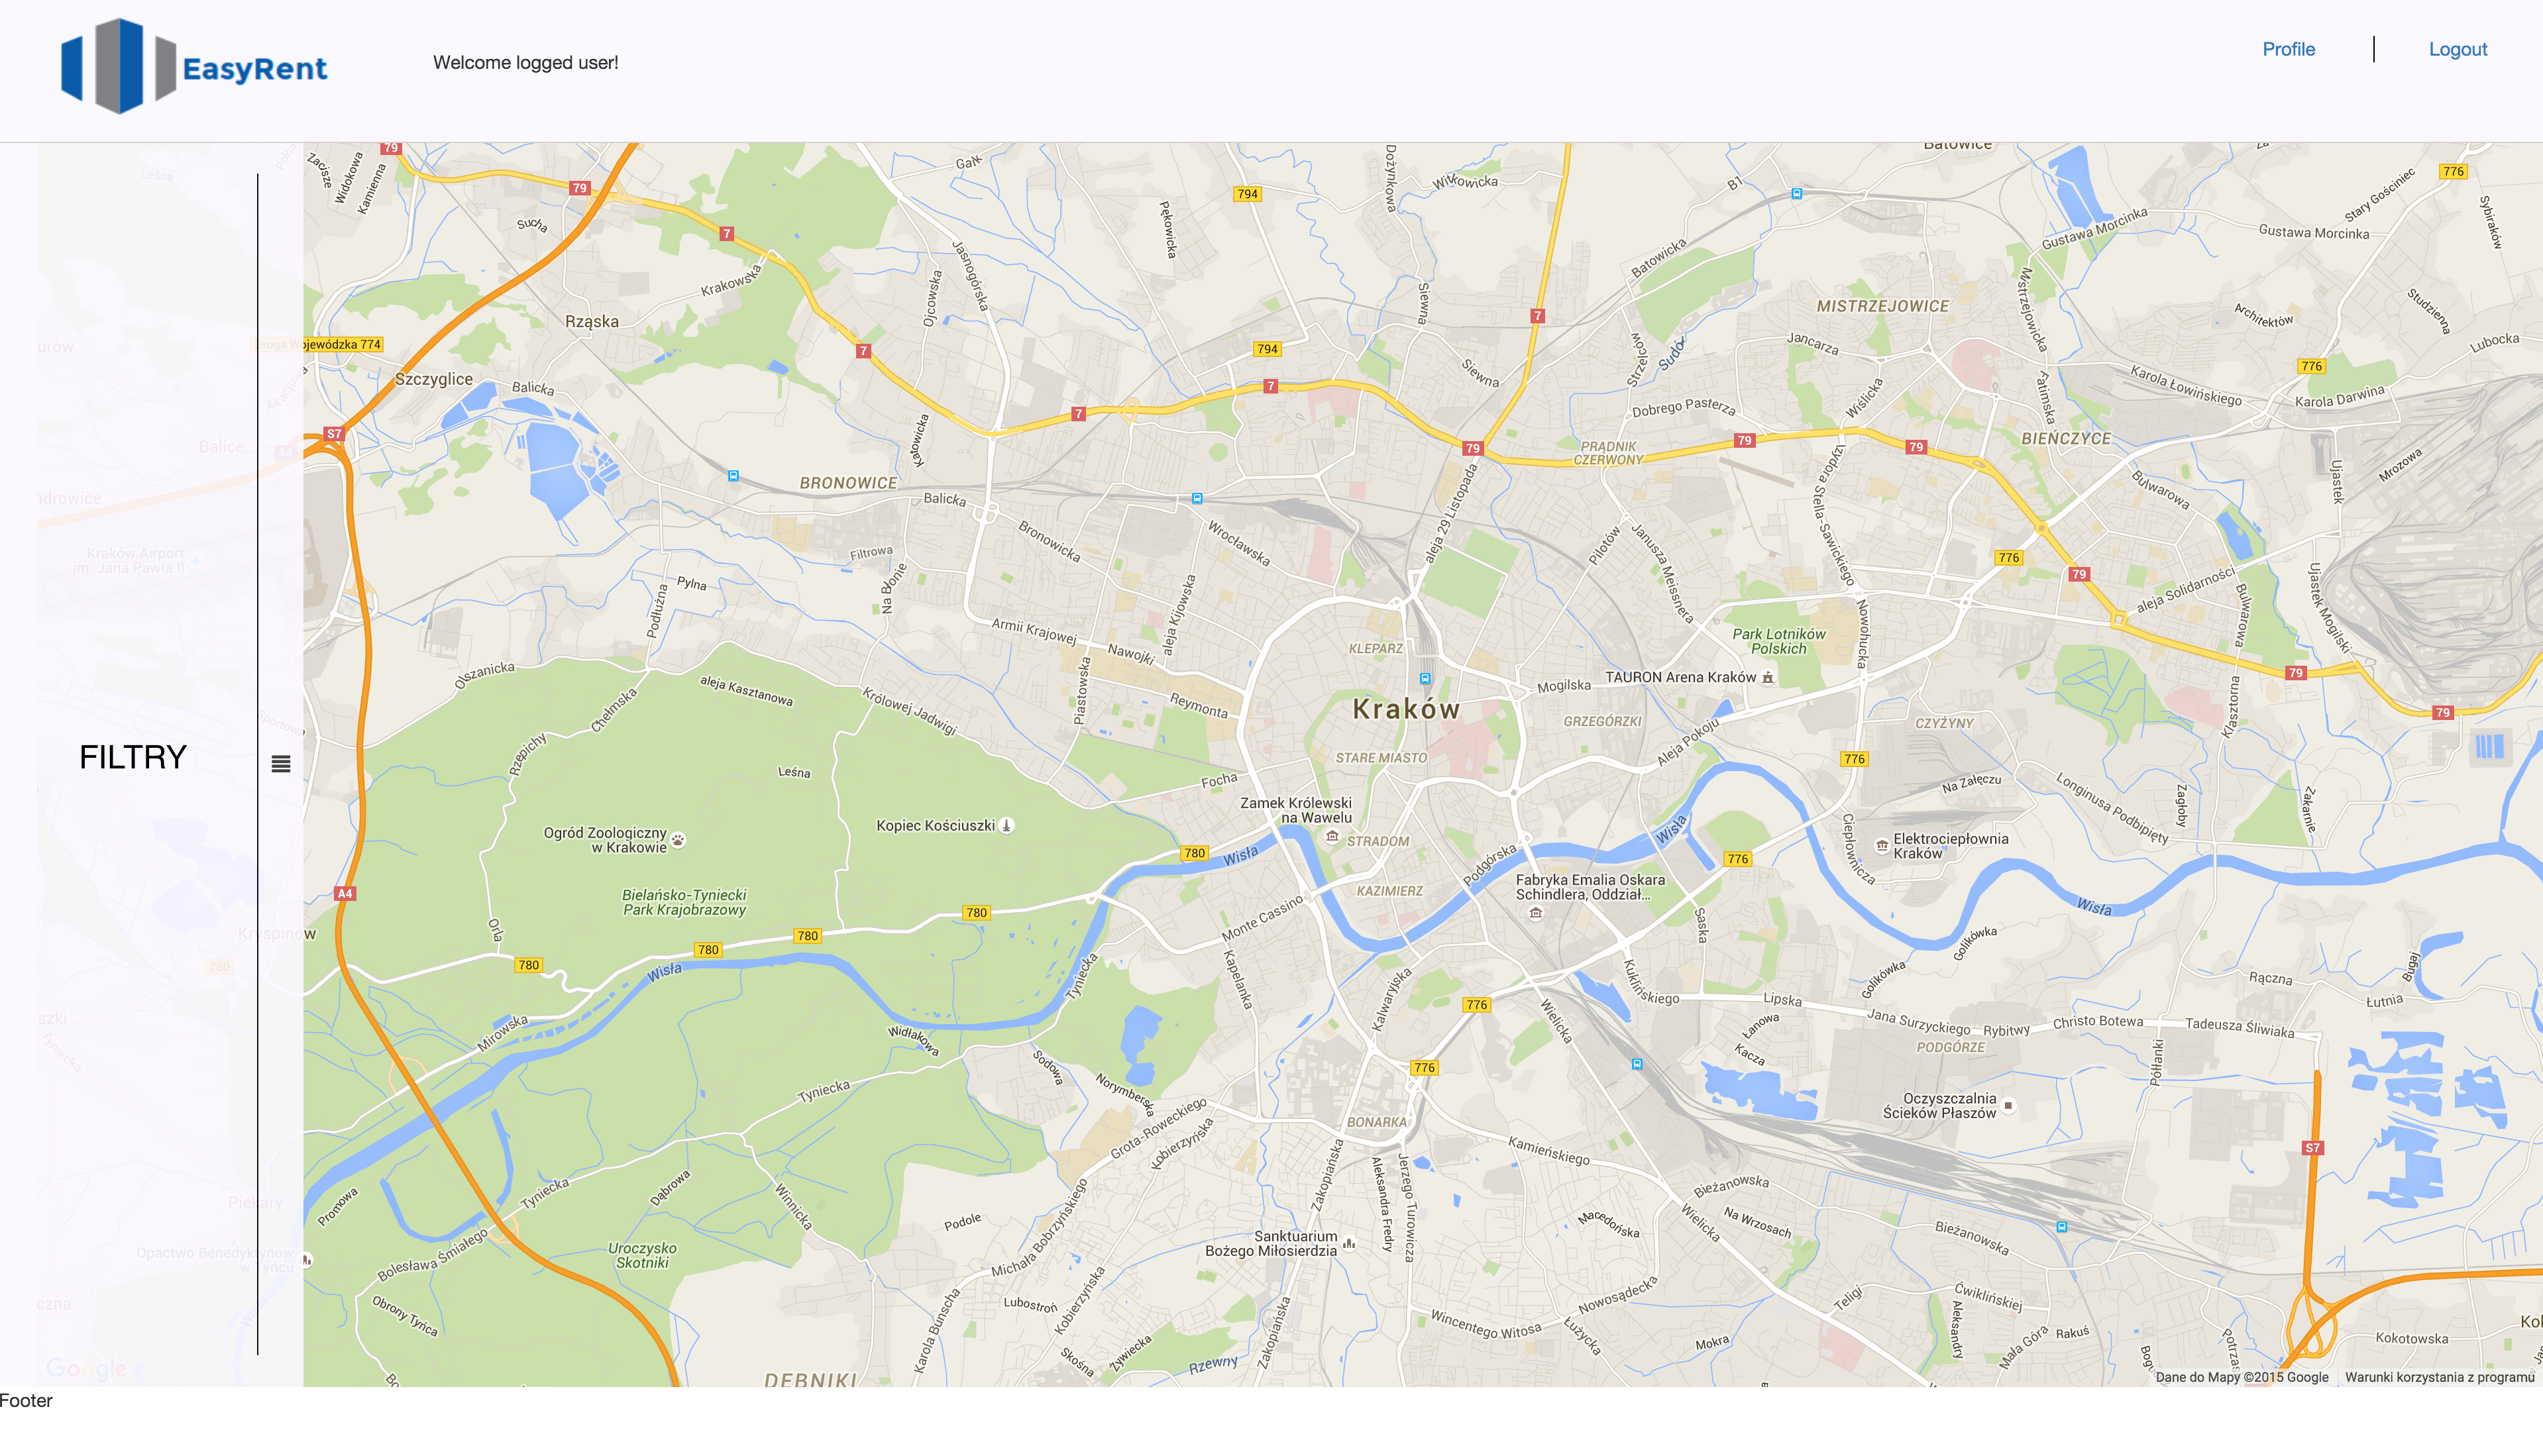
\includegraphics[scale=0.15]{pictures/after_login.png}}
\end{frame}

%---------------------------------------------------------------------------


\end{document}

